%
% schnittkruemmung.tex
%
% (c) 2017 Prof Dr Andreas Müller, Hochschule Rappersewil
%
\section{Schnittkrümmung}
\rhead{Schnittkrümmung}
Die Krümmung von Kurven kann dazu verwendet werden, Flächen im
dreidimensionalen Raum zu analysieren.

\subsection{Flächen}
Wir betrachten in den folgenden Abschnitten Flächen, die durch zwei
Parameter $u,v\in\mathbb R^2$ parametrisiert sind.

\begin{definition}
Eine Abbildung
\[
g\colon \Omega\to\mathbb R^3: (u,v)\mapsto g(u,v),
\]
wobei $\Omega\subset\mathbb R^2$
eine offene Teilmenge von $\mathbb R^2$ ist, heisst eine Fläche.
\end{definition}

\begin{beispiel}
Sei eine Funktion $f(x,y)$ von zwei Variablen gegeben.
Dann ist die Funktion
\[
g\colon\mathbb R^2\to \mathbb R^3
: (x,y)\mapsto (x,y,f(x,y))
\]
eine Fläche.
Sie heisst auch der Graph der Funktion $f(x,y)$.
\end{beispiel}

Jede Fläche enthält zwei Scharen von Kurven, die durch die Koordinaten $u$
bzw.~$v$ parametrisiert sind, wir nennen sie die Koordinatenlinien.
Zu jedem $v$-Wert $v_0$ gibt es eine $u$-Koordinatenlinie
\[
c_{v_0}
\colon
\mathbb R \to \mathbb R^2
:
u\mapsto
c_{v_0}(u) = g(u, v_0)
\]
und zu jedem $u$-Wert $u_0$ gibt es eine $v$-Koordinatenlinie
\[
c_{u_0}
\colon
\mathbb R \to \mathbb R^2
:
v\mapsto
c_{u_0}(v) = g(u_0, v).
\]

\begin{beispiel}
Die Oberfläche der Einheitskugel im dreidimensionalen Raum kann mit
geographischer Länge $\lambda$ und geographischer Breite $\varphi$
parametrisiert werden.
Die Funktion $g(\lambda,\varphi)$ hat die Form
\begin{equation}
g(\lambda,\varphi)
=
\begin{pmatrix}
\sin\varphi\cos\lambda\\
\sin\varphi\sin\lambda\\
\cos\varphi
\end{pmatrix},\qquad
-\pi \le \lambda \le \pi,\quad
-\frac{\pi}2 \le \varphi \le \frac{\pi}2
.
\end{equation}
Die Koordinatenlinien auf einer Kugeloberfläche sind wohlbekannt. 
Die Koordinatenlinie zu einem vorgegebenen $\varphi_0$ wird durch
$\lambda$ parametrisiert und hat die Form
\[
\lambda
\mapsto
\begin{pmatrix}
\sin\varphi_0\cos\lambda\\
\sin\varphi_0\sin\lambda\\
\cos\varphi_0
\end{pmatrix},\qquad -\pi\le\lambda\le\pi,
\]
dies ist ein Breitenkreis.
Die Koordinatenlinie zu einem vorgegebenen $\lambda_0$ wird durch
$\varphi$ parametrisiert und hat die Form
\[
\varphi
\mapsto
\begin{pmatrix}
\sin\varphi\cos\lambda_0\\
\sin\varphi\sin\lambda_0\\
\cos\varphi
\end{pmatrix},\qquad -\frac{\pi}2 \le \varphi\le \frac{\pi}2,
\]
dies ist ein Längenkreis.
Man beachte, dass Werte $-\frac{\pi}2\le \varphi \le \frac{\pi}2$ nur einen
Halbkreis zwischen Süd- und Nordpol beschreiben.
\end{beispiel}

Wir betrachten jetzt den Punkt $P=g(u_0,v_0)$ auf der Fläche.
Zu jedem Flächenparameter gibt es einen Tangentenvektor, den man durch
Ableitung nach dem Parameter bekommen kann:
\begin{equation}
t_u
=
t_u(P)
=
t_u(u_0,v_0)
=
\frac{\partial g(u_0,v_0)}{\partial u},
\qquad
t_v
=
t_v(P)
=
t_v(u_0,v_0)
=
\frac{\partial g(u_0,v_0)}{\partial v}.
\end{equation}
Aus diesen Tangentialvektoren lässt sich auch der Normalenvektor
\begin{equation}
n(P) = n(u_0,v_0) = t_u(u_0,v_0) \times t_v(u_0,v_0)
\end{equation}
bestimmen.
Damit die beiden Tangentialvektoren und der Normalenvektor wohldefiniert sind,
müssen wir verlangen, dass die partiellen Ableitungen von $g$ nach $u$ und $v$
wohldefiniert sind und nicht verschwinden.
Daher soll im Folgenden immer angenommen sein, dass $g$ genügend oft stetig
differenzierbar ist, und dass die ersten Ableitungen nach den Flächenparametern
nicht verschwinden.

\subsection{Schnittkurven}
\begin{figure}
\centering
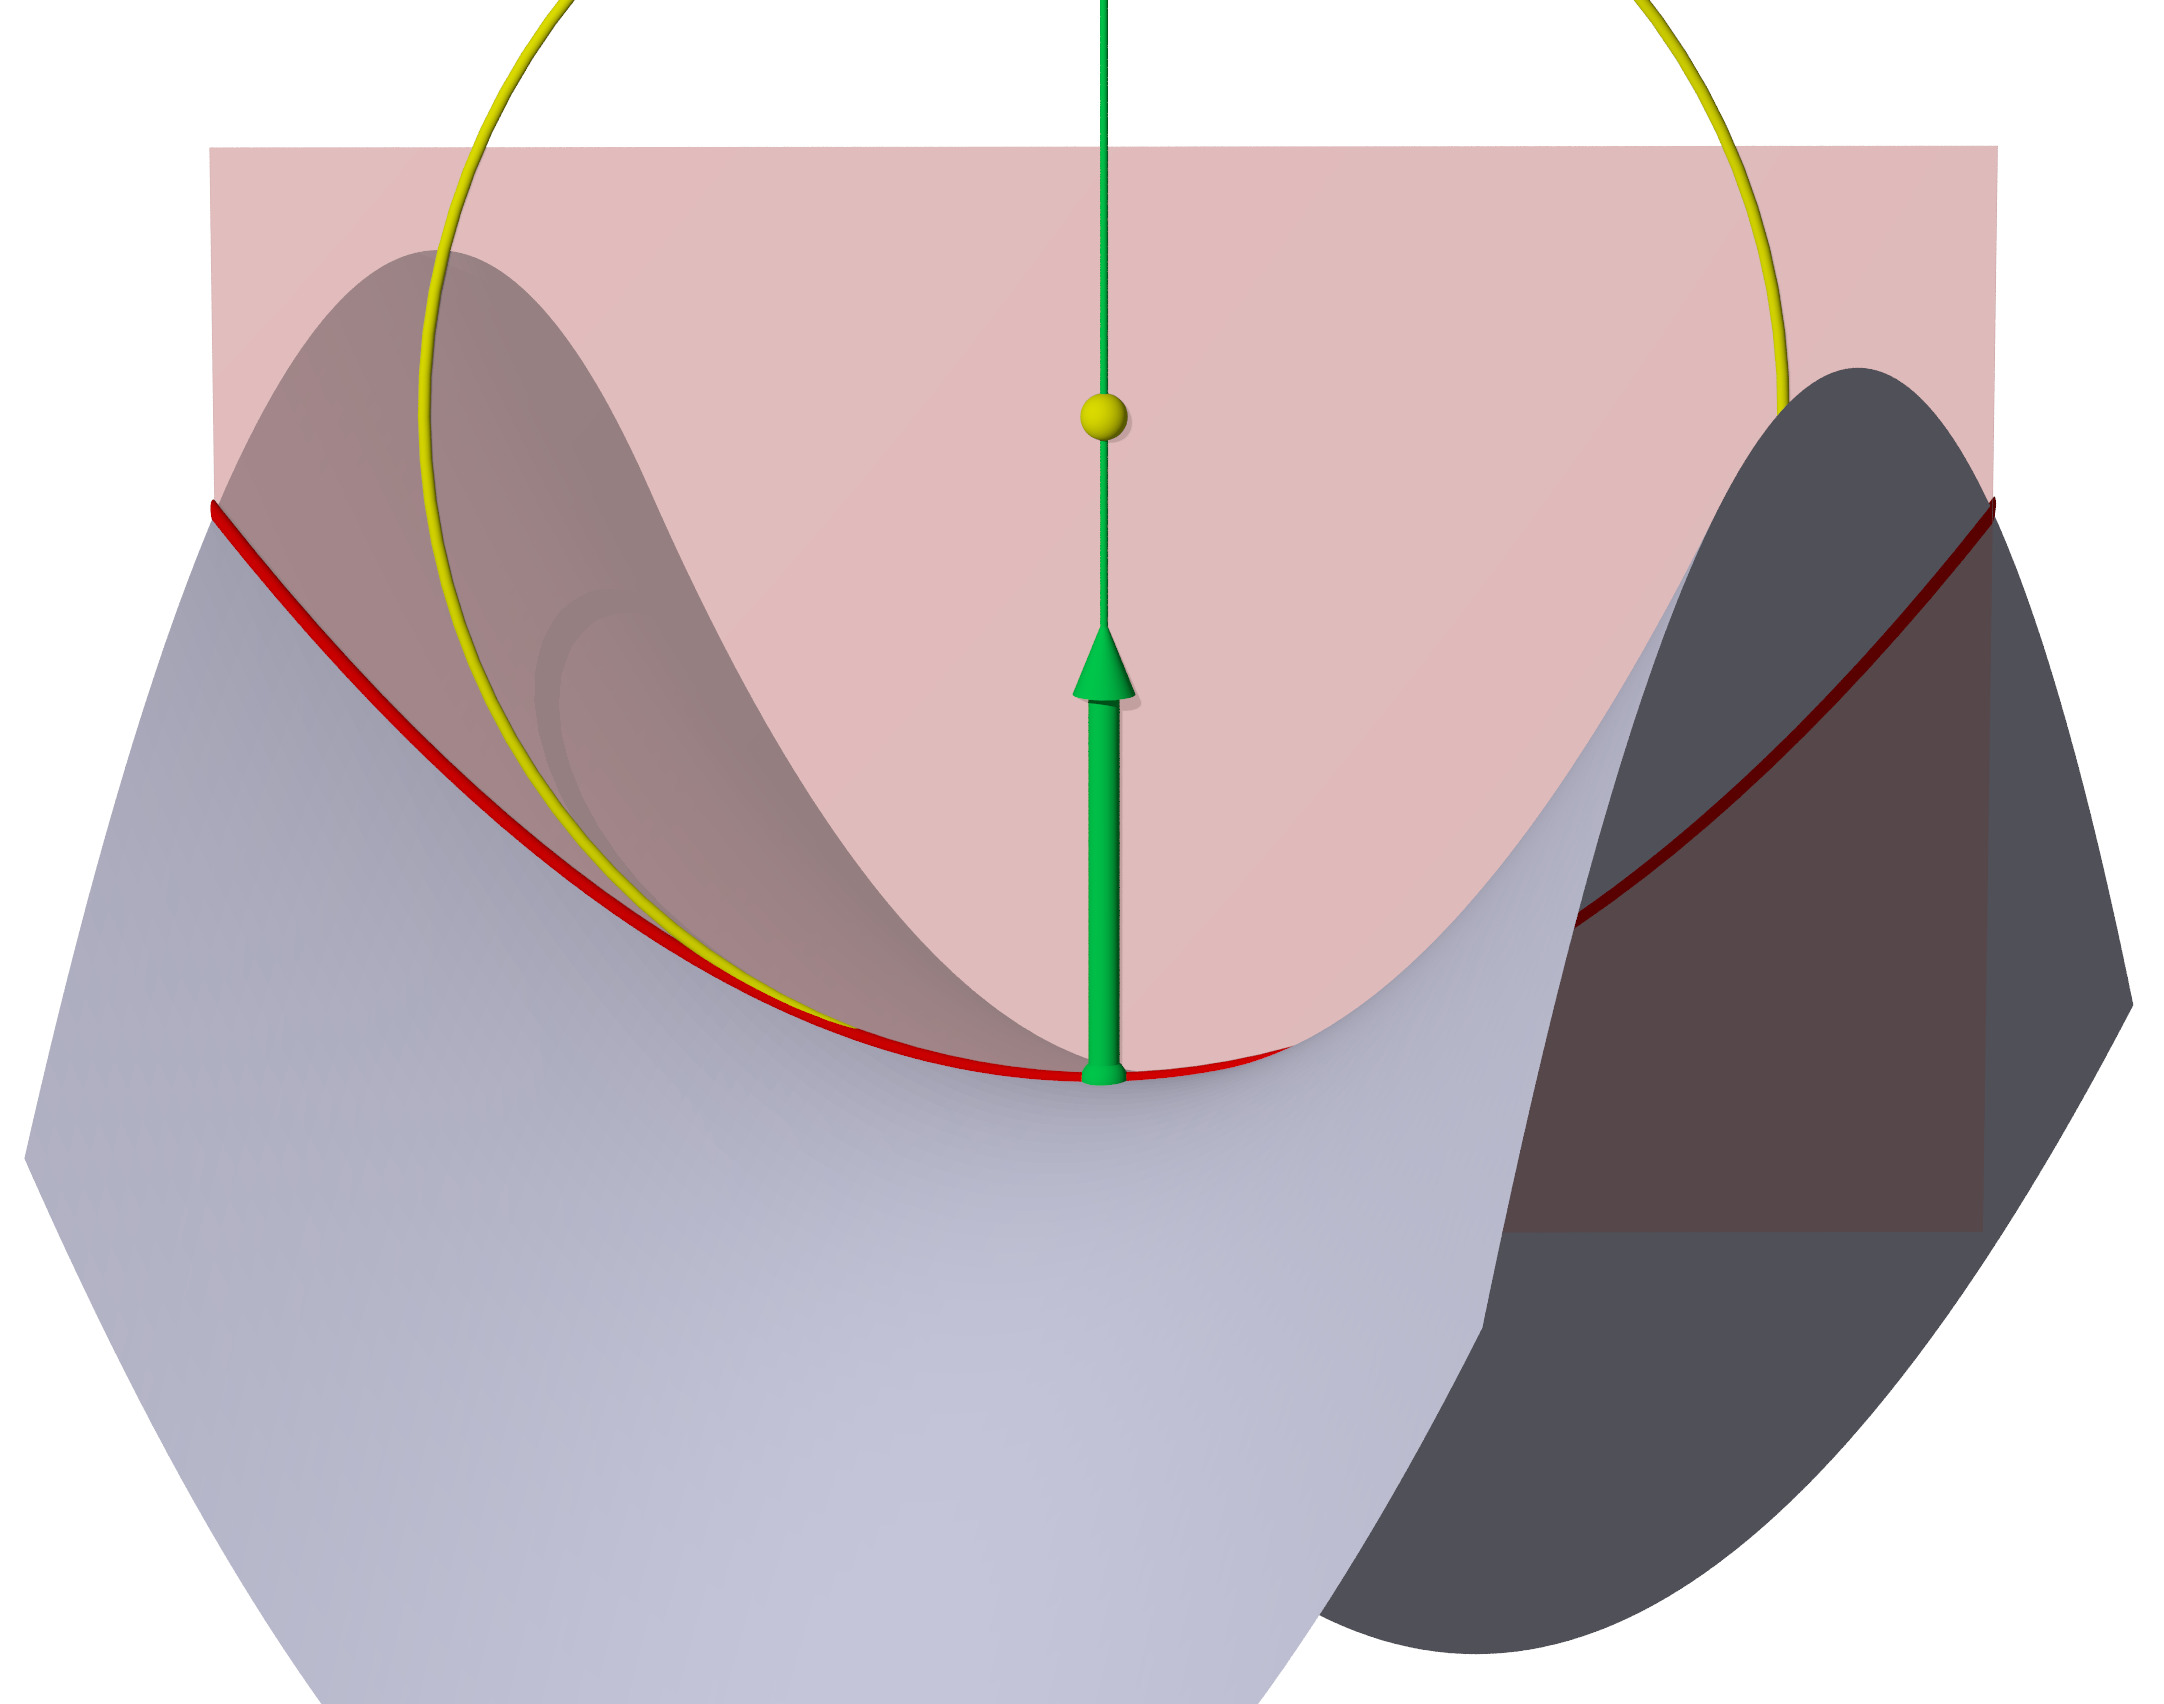
\includegraphics[width=\hsize]{chapters/3d/schnittkruemmung.jpg}
\caption{Die Schnittkrümmung einer Fläche $g(u,v)$ im Punkt $P$ ist
die Krümmung der Schnittkurve (rot) einer Ebene durch $P$, die den
Normalenvektor $n(P)$ (grün) enthält.
Der Krümmungskreis und sein Mittelpunkt $Q$ sind gelb eingezeichnet.
\label{skript:schnittkruemmung}}
\end{figure}
Sei jetzt also eine Fläche $g(u,v)$ gegeben.
Im Punkt $P=g(u_0,v_0)$ betrachten wir Ebenen, die die Normale $n(P)$
enthalten.
Die Schnittkurve der Fläche mit einer solchen Ebene ist eine ebene
Kurve, wir können also deren Krümmung bestimmen
(Abbildung~\ref{skript:schnittkruemmung}).
Der Mittelpunkt $Q$ des Krümmungskreises liegt auf der Normalen
und ist daher von der Form $Q = P + \varrho \cdot n(P)$.
Im Gegensatz zur Berechnung der Krümmung in
Abschnitt~\ref{section:kurve:kruemmung}, die immer eine Zahl $\ge 0$
als Wert der Krümmung geliefert hat, spielt es hier das Vorzeichen von
$\varrho$ eine Rolle.
Ist die Kurve in Richtung von $n(P)$ gekrümmt, liegt der Punkte $Q$ auf der
gleichen Seite der Fläche wie $n(P)$ und damit $\varrho\ge 0$.
Ist dagegen die Kurve in die Gegenrichtung von $n(P)$ gekrümmt, liegt der
Punkt $Q$ auf der anderen Seite und damit ist $\varrho\le 0$.
Der Punkt $Q$ und der Krümmungskreis sind in
Abbildung~\ref{skript:schnittkruemmung} gelb eingezeichnet.

\begin{beispiel}
\label{skript:sattelbeispiel}
Als Beispiel berechnen wir die Krümmung der Schnittkurve des Graphen
der Funktion
$f(x,y) = x^2-y^2$ im Nullpunkt.
Die Normale $n(0)$ ist der Einheitsvektor in $z$-Richtung, die Schnitt\-ebene
enthält also die $z$-Achse.
Die zulässigen $x$- und $y$-Werte auf der Schnittgeraden sind daher Vielfache
eines Einheitsvektors in der $x$-$y$-Ebene, zum Beispiel $x=t\cos\alpha$
und $y=t\sin\alpha$.
Der Wert von $z$ ist dann
\[
z(t)
=
f(x,y)
=
f(t\cos\alpha,t\sin\alpha)
=
t^2\cos^2\alpha - t^2\sin^2\alpha
=
t^2(\cos^2\alpha - \sin^2\alpha)
=
t^2\cos 2\alpha.
\]
Da der Tangentialvektor ein Einheitsvektor ist, ist $t$ die Länge entlang
der tangentialen Achse in der Schnittebene.
Die Koordinate $z$ hängt davon quadratisch von $t$ ab.
Die Krümmung im Nullpunkt kann daher mit der
Formel~\eqref{skript:kruemmung:parabel:scheitel}
berechnet werden, wir finden
\begin{equation}
\kappa = 2\cos2\alpha
\qquad\Rightarrow\qquad
\varrho = \frac1{2\cos2\alpha}.
\label{skript:kruemmung:sattel}
\qedhere
\end{equation}
\end{beispiel}

Selbstverständlich ist es mit entsprechendem Aufwand möglich, allgemeine
Formeln für die Krümmung der Schnittkurven herzuleiten.
Da wir solche aber nicht explizit brauchen, sondern nur einige wenige
spezielle Eigenschaften, vor allem die Richtungsabhängigkeit, verzichten
wir darauf, diesen Formelapparat zu entwickeln.

\subsection{Richtungsabhängigkeit%
\label{skript:kruemmung:richtungsabhaengigkeit}}
Im Beispiel auf Seite~\pageref{skript:sattelbeispiel} wurde gezeigt, wie
die Krümmung der Schnittkurve von der Richtung der Schnittebene
abhängt.
Dabei entstand die einfache Formel~\eqref{skript:kruemmung:sattel}.
In diesem Abschnitt möchten wir zeigen, dass eine ähnlich einfache
Formel für jede beliebige Fläche gilt.

Gegeben ist also eine Fläche mit Parametrisierung $g(u,v)$, wir möchten
die Krümmungen im Punkte $P=g(u_0,v_0)$ genauer untersuchen.
Offenbar spielt dafür die Lage der Fläche im Raum keine Rolle, wir können
also in einem ersten Schritt das Koordinatensystem so drehen, dass der
Punkt $P$ in den Nullpunkt zu liegen kommt, und dass die $x$-$y$-Ebene des
Koordinatensystems tangential an die Fläche wird.
In dieser Lage lässt sich die Fläche in der Umgebung des Punktes $P$
immer als Graph einer Funktion
$z=f(x,y)$ schreiben\footnote{%
Der exakte Beweis dieser intuitiv einleuchtenden Aussage kann mit
dem Satz über implizite Funktionen erfolgen, wir wollen auf die Details
verzichten.}.
Damit haben wir das Problem auf die viel einfachere Situation eines
Graphen reduziert.

Die Funktion $f(x,y)$ kann man als Taylorreihe schreiben, wovon wir nur
die ersten drei Terme hinschreiben wollen
\begin{align*}
f(x,y)
&=
\frac{\partial^2 f}{\partial x^2}x^2
+
2\frac{\partial^2 f}{\partial x\partial y}xy
+
\frac{\partial^2 f}{\partial y^2}y^2
+
o(x^2+y^2)
\\
&=
ax^2 + 2bxy + cy^2 + o(x^2+y^2).
\end{align*}
Die Normale auf die Fläche ist die $z$-Achse, die Schnittebene kann
daher wie im Beispiel wieder durch
\[
x=t\cos\alpha,\quad y=t\sin\alpha
\]
beschrieben werden.
Die Schnittkurve in der Schnittebene hat die Gleichung
\begin{equation}
z
=
(a\cos^2\alpha + 2b\cos\alpha\sin\alpha  + c\sin^2\alpha)t^2
+
\text{Terme dritter Ordnung in $t$}.
\label{skript:kruemmung:klammer}
\end{equation}
Bei der Berechnung der Krümmung braucht man nur die ersten und zweiten
Ableitungen. 
Die erste Ableitung ist ohnehin $0$, die zweiten wird durch die Klammer
im Ausdruck \eqref{skript:kruemmung:klammer} gegeben.
Die Terme dritter Ordnung bleiben nach zweimaligem Ableiten Terme erster
Ordnung, für den Wert $t=0$ fallen sie also weg.
Es bleibt also der quadratische Term als krümmungsbestimmend, wir
können die Formel~\eqref{skript:kruemmung:parabel:scheitel} verwenden, um die
Krümmung in Abhängigkeit von $\alpha$ zu ermitteln.
Wir erhalten
\begin{equation}
\kappa(\alpha)
=
2(a\cos^2\alpha + 2b\cos\alpha\sin\alpha + c\sin^2 \alpha)
=
2\biggl(
\frac{\partial^2 f}{\partial x^2}\cos^2\alpha
+
2\frac{\partial^2 f}{\partial x\partial y}\cos\alpha\sin\alpha
+
\frac{\partial^2 f}{\partial y^2}\sin^2 \alpha
\biggr).
\label{skript:kurve:kruemmungalpha}
\end{equation}
Die Krümmung einer Schnittkurve in Richtung des Tangentialvektors
$(\cos\alpha,\sin\alpha)$ ist daher durch die zweiten Ableitungen von
$f$ im Punkt $P$ vollständig bestimmt.

\begin{definition}
In jedem Punkt gibt es also eine Abbildung, die jedem
Tangentialeinheitsvektor $e$
die Krümmung der Schnittkurve $\kappa(e)$ einer Ebene durch den Normalenvektor
$n(P)$ und die Tangentenrichrtung $e$ mit der Fläche zuordnet.
Sie heisst die Schnittkrümmung der Fläche in Richtung $e$.
Das Vorzeichen von $\kappa(e)$ ist so gewählt, dass $P+n(P)/\kappa(e)$ der
Mittelpunkt des Krümmungskreises ist.
\end{definition}

\subsection{Mittlere Krümmung%
\label{skript:kurve:mittlerekruemmung}}
Aus dem Ausdruck~\eqref{skript:kurve:kruemmungalpha}
für $\kappa(\alpha)$ kann man jetzt auch den Mittelwert
der Krümmung für alle Richtungen berechnen.
Dazu berechnet man
\begin{align*}
M
&=
\frac{1}{2\pi}\int_0^{2\pi} \kappa(\alpha)\,d\alpha
\\
&=
2\cdot
\frac{1}{2\pi}\int_0^{2\pi}
a\cos^2\alpha + 2b\cos\alpha\sin\alpha + c\sin^2 \alpha
\,d\alpha
\\
&=
2\cdot\biggl( \frac{a}2 + \frac{c}2\biggr)
=
a+c
=
\frac{\partial^2 f}{\partial x^2}
+
\frac{\partial^2 f}{\partial y^2}
=
\operatorname{Spur}H
=
\Delta f.
\end{align*}
Darin wurde
\begin{align*}
\frac1{2\pi}\int_0^{2\pi}\cos^2\alpha\,d\alpha
&=
\frac1{2\pi}\int_0^{2\pi}\sin^2\alpha\,d\alpha
=
\frac12
\qquad\text{und}\qquad
\\
\frac{1}{2\pi}\int_0^{2\pi}2\sin\alpha\cos\alpha\,d\alpha
&=
\frac{1}{2\pi}\int_0^{2\pi}\sin2\alpha\,d\alpha
=
0
\end{align*}
verwendet.
Der Mittelwert der Krümmung ist also die Spur der Hessischen Matrix
(Siehe auch Abschnitt~\ref{skript:kurven:section:hauptkruemmungen}).

\begin{definition}
\label{skript:definition:mittlerekruemmung}
Die {\em Mittlere Krümmung} $M$ ist der Mittelwert der Schnittkrümmung
$\kappa(\alpha)$ über alle Winkel $\alpha$.
\end{definition}

Man beachte, dass die Beziehung $M=\operatorname{Spur}H$ nur 
im Nullpunkt gilt und nur dann, wenn die Fläche im Nullpunkt tangential
an die $x$-$y$-Ebene verläuft.




